\model{Search Trees}

%TODO replace images from textbook (Copyrighted by Pearson -- fair use?)

\begin{center}
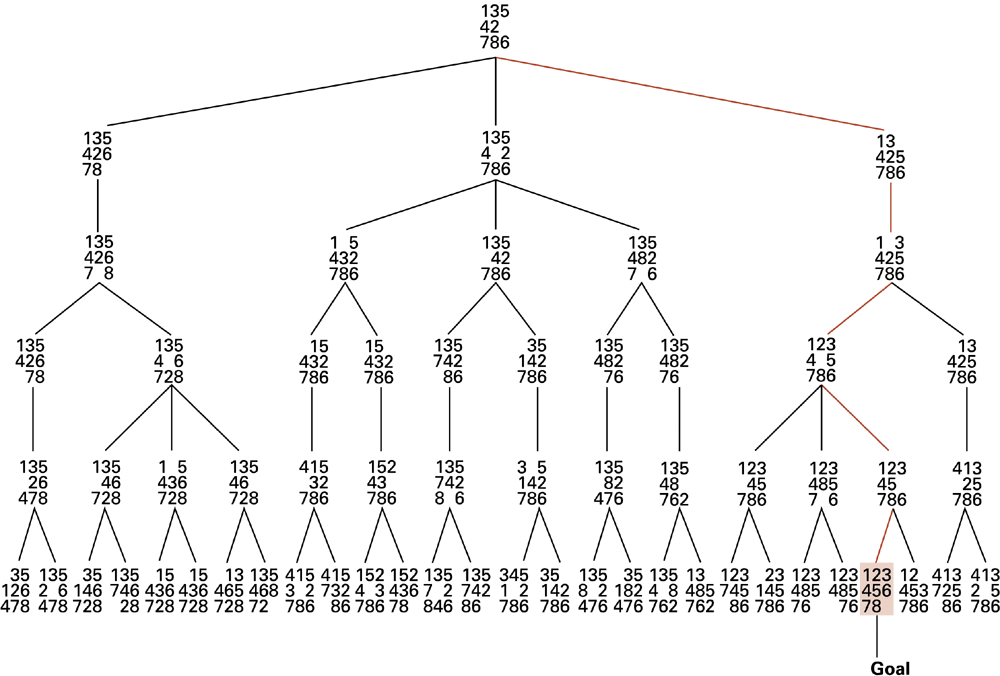
\includegraphics[width=0.9\textwidth]{CSP/search-tree1.png}
\end{center}


\quest{15 min}


\Q In your own words, describe what the above diagram represents.

\begin{answer}
It shows all possible configurations of the 8-tile game, one move at a time, starting from the top configuration until the goal is reached.
\end{answer}


\Q Given that there are always at least two possible moves, why do some board configurations seem to have only one branch?

\begin{answer}
The lines are bidirectional: you can move up or down the tree.
In the case of one branch, moving one tile moves you down the tree and moving the other moves you back up.
\end{answer}


\Q \label{guess} Consider two methods for making the move choices at each step:
\emph{Random} (just choose randomly among all legal moves), and
\emph{Lowest} (always choose the lowest numbered available tile to move).
Could either of these methods get to a solution?

\begin{answer}
They wouldn't work well, depending on the initial configuration.
But you might get lucky if the puzzle is easy enough to solve.
\end{answer}


\Q If you were given several puzzle layouts and had to choose the easiest to solve, how would you choose?

\begin{answer}
I would pick the one that was closest to the goal.
In other words, the one that would require the fewest number of moves.
\end{answer}


\Q \label{heurs} Describe an algorithm that can take any 8-Puzzle grid and compute some measure of the difficulty.
Use your thinking from the previous question: think about how to get to a number that is bigger, the harder the puzzle might be to solve.

\begin{answer}
One simple algorithm is to count the number of tiles that are out of place.
A more complex example is to measure how many positions each tile is away from its final position.
\end{answer}


\Q Apply your algorithm to the second row of the model. You should get a number for each of the three board configurations.

\begin{answer}[6em]
Using the ``number of tiles out of place'' algorithm, the first board has 4, the second has 6, and the third has 4.
\end{answer}


\Q Describe how you could use your algorithm from \ref{heurs} to make a better next-step choice method than the methods in \ref{guess}.

\begin{answer}
Compute the difficulty of each option, and select the one with the least difficulty.
If there is a tie, pick the one with the lowest tile.
\end{answer}
